\section{Autómatas y Redes de Petri}

\subsection{Autómatas o Máquinas de Estado}

Existen muchas formas de modelar el comportamiento de los sistemas, y el uso de
máquinas de estado finitas es una de las más antiguas y más conocidas.
Las máquinas de estado finitas o autómatas nos permiten pensar acerca del
``estado'' de un sistema en un instante en particular y caracterizar el comportamiento de dicho
sistema basado en ese estado. El uso de esta técnica de modelado no está
limitada al desarrollo de sistemas de software.\cite{FSM_Wright}

\subsubsection{Definición Conceptual de Máquina de Estado}

Si una máquina de estados M, en un instante dado, se encuentra en el estado
$E_{0}$ y ocurre un evento $e_{0}$ que lleva a M al estado $E_{1}$, se
dice que ocurrió una \textit{transición} del estado $E_{0}$ al estado
$E_{1}$.
A partir de esto se puede deducir que M no puede estar en $E_{0}$ y $E_{1}$
a la vez, y por lo tanto los estados de una máquina de estados, son
\textbf{estados globales} del sistema modelado.

Analizando la semántica de las máquinas de estado, se pueden
identificar algunas características clave de un sistema que puede ser modelado con máquinas de
estados finitas:
\begin{itemize}
  \item El sistema debe ser descripto por conjunto finito de estados.
  \item El sistema debe tener una cantidad finita de entradas y/o eventos que
  puedan disparar transiciones entre estados.
  \item El comportamiento del sistema en un instante dado depende del estado
  actual y de sus entradas o eventos que ocurran en ese instante.
  \item Para cada estado posible en que el sistema pueda encontrarse existe un
  comportamiento definido para cada posible entrada o evento.
  \item El sistema tiene un estado inicial único y definido.
\end{itemize} \cite{FSM_Wright}

\subsubsection{Definición Formal de Máquina de Estado}

A fin de eliminar la ambigüedad existente en una definición conceptual, se
introduce una definición formal de Autómata Finito:
\newline\newline\emph{Definición:} Un autómata finito M está definido por una
tupla $(\Sigma, Q, q_{0}, F, \sigma)$, donde:
\begin{itemize}    
  \item $\Sigma$ es el conjunto de símbolos de entrada de M
  \item $Q$ es el conjunto de estados de M
  \item $q_{0}$ es el estado inicial de M
  \item $F \subseteq Q$ es el conjunto de estados finales de M
  \item $\sigma : Q  \times \Sigma \rightarrow Q$ es la función de
  transición
\end{itemize} \cite{FSM_Wright}

\subsection{Redes de Petri}

Tomando el concepto de transición en una máquina de estados, se lo puede
extender a una entidad propia.
Esta transitión $t_{i}$ será denotada por una barra, un rectángulo o un
cuadrado, y puede tener múltiples arcos de entrada (entrantes) y de salida
(salientes) a la vez. Esta transición, representa la \textit{transición} básica
de una Red de Petri (RdP).\cite{PetriNetsFundamentals}

De la misma forma que en una máquina de estados los círculos denotan estados
del sistema, en una RdP se utilizan círculos para denotar las \textit{plazas} o
\textit{lugares} de la red. Estas plazas no representan estados globales, sino
\textbf{estados locales}. \cite{PetriNetsFundamentals}

El estado local de una plaza, está dado por la cantidad de \textit{tokens} o
\textit{marcas} que esta contiene.

Como consecuencia de su estructura, una Red de Retri puede ser representada como
un grafo bipartito, donde los tipos de nodo existentes son \textit{plazas} y
\textit{transiciones}. Estos nodos se unen entre dos de distinto tipo
únicamente (de ahí el calificativo de bipartito), utilizando \textit{arcos}.\\

\begin{figure}[h]
	\centering
	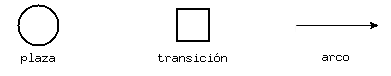
\includegraphics[width=75mm]{Partes_De_Una_Red}
	\caption{Partes de una Red de Petri}
	\label{fig:partes_de_una_red}
\end{figure}

Se pueden visualizar las partes de una Red de Petri en la figura
\ref{fig:partes_de_una_red}.\\


\begin{figure}[h]
    \centering
    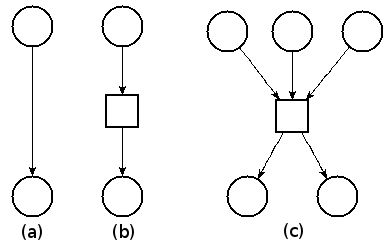
\includegraphics[height=40mm]{Automata_Y_Petri}
    \caption{Equivalencia entre una Máquina de Estados y una Red de Petri}
    \label{fig:automata_y_petri}
\end{figure}

En la figura \ref{fig:automata_y_petri} se aprecia:\\
\begin{itemize}
  \item[(a)] Una máquina de estados de dos estados y una transición.
  \item[(b)] Una RdP equivalente a la máquina de (a).
  \item[(c)] Una RdP con una transición con múltiples arcos de entrada y de
  salida.
\end{itemize}

Se puede extraer como consecuencia directa de esta extensión de la semántica de
un autómata que en una Red de Petri:
\begin{itemize}
  \item Múltiples tokens pueden existir en el modelo al mismo tiempo, y
  particularmente en una plaza.
  \item No existe un estado global explícito.
  \item El estado global del sistema es el conjunto de todos los estados
  parciales, representados por las plazas y sus tokens. A este conjunto se lo
  llama el \textbf{marcado} de la red.
\end{itemize}

\subsubsection{Definición Formal de Red de Petri}
A fin de eliminar ambigüedades, se presenta una serie de definiciones sobre
Redes de Petri.

\begin{itemize}
  \item [\underline{Definición 1}:] Una Red de Petri R está definida por la
  tupla $(P, T, Pre, Post)$ donde:
  \begin{itemize}
    \item $ P = \{ p_1, p_2, \ldots, p_p \} $ un conjunto de plazas.\footnote{Se
    utiliza $p$ como la cantidad de plazas de la RdP en todo momento dentro de este informe por simplicidad para el lector}
    \item $ T = \{ t_1, t_2, \ldots, t_t \} $ un conjunto de transiciones, donde
    $ P \cap T = \emptyset $. \footnote{Se utiliza $t$ como la cantidad de
    transiciones de la RdP en todo momento dentro de este informe por
    simplicidad para el lector}
    \item $ Pre: P \times T \rightarrow \mathbb{N}^{p} $ aplicación de
    precedencia.\footnote{Se toma la definición de números naturales incluyendo
    el cero por simplicidad de notación.}
    \item $ Post: P \times T \rightarrow \mathbb{N}^{p} $ aplicación de
    incidencia.
  \end{itemize}
  $ Pre (p_i, t_j) $ contiene el peso del arco que va de $ p_i $ a $ t_j $, y
  $ Post (p_i, t_j) $ contiene el peso del arco que va de $ t_j $ a $ p_i $

  \item [\underline{Definición 2}:] Una Red de Petri Marcada está
  definida por el par $(R, M)$, donde R es una RdP y $ M : P \rightarrow
  \mathbb{N}^{p} $ (siendo $P$ el conjunto de plazas de dimensión $n$) es una aplicación llamada \textit{marcado}.\\
  $m(R)$, o más simplemente $m$ si la red es conocida, define el marcado de la
  RdP y $m(p_{i})$ o $mp_{i}$ indica el marcado de la plaza $p_{i}$, es decir,
  el número de tokens contenido en la plaza $p_{i}$.\\
  La marca inicial se denota $m_{0}$ y da la cantidad inicial de tokens en todas
  las plazas de la red, por lo que especifica el estado inicial del sistema.
  
  \item [\underline{Definición 3}:] Para una marca $m$, una transición $t_{j}$
  está sensibilizada, y por lo tanto es disparable, si y solo si:\\
  $$ \forall p_{i} \in P, m(p_i) \geq Pre(p_{i}, t_{j}) $$
  Conceptualmente, una transición está sensibilizada si todas sus plazas de
  entrada contienen al menos la cantidad de tokens que indica el peso de los
  arcos que las unen.

  En la figura \ref{fig:transiciones_no_sensibilizadas} se observa gráficamente esta definición mediante dos casos de transiciones no sensibilizadas. Nótese
  el peso de los arcos.

  \begin{figure}[h]
    \centering
    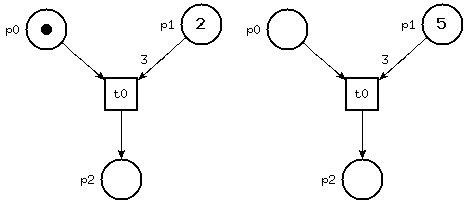
\includegraphics[height=40mm]{Transiciones_No_Sensibilizadas}
    \caption{Ejemplos de transiciones no sensibilizadas.}
    \label{fig:transiciones_no_sensibilizadas}
  \end{figure}
  
  \item [\underline{Definición 4}:] La estructura de una Red de Petri
  se denota $ N = \{P, T, F, W\} $ donde,
  \begin{itemize}
    \item $P$ es en conjunto de plazas.
    \item $T$ es el conjunto de transiciones, donde se cumple que $ P \cap T =
    \emptyset $
    \item $F$ es el conjunto de arcos, donde se cumple que $ F \subseteq (P
    \times T) \cup (F \times P) $.
    \item $W$ es la función de peso de los arcos.
  \end{itemize}

  \item [\underline{Definición 5}:] Conjunto de transición y plaza de entrada y
  de salida.
  \begin{itemize}
    \item[] El conjunto de las plazas de entrada a la transición $t$ se denota
    $\bullet t$ y se define,
    $$ \bullet t = \{ p \in P : (p, t) \in F \} $$
    \item[] El conjunto de las plazas de salida de la transición $t$ se denota $
    t \bullet$ y se define,
    $$ t \bullet = \{ p \in P : (t, p) \in F \} $$
    \item[] El conjunto de las transiciones de entrada a la plaza $p$ se
    denota $\bullet p$ y se define,
    $$ \bullet p = \{ t \in T : (t, p) \in F \} $$
    \item[] El conjunto de las transiciones de salida de la plaza $p$ se denota
    $ p \bullet$ y se define,
    $$ p \bullet = \{ t \in T : (p, t) \in F \} $$
  \end{itemize}
\end{itemize}

\subsubsection{Disparo de una Transición}

La condición de disparo relacionada a $Pre(p_{i}, t_{j})$ significa que para
todas las plazas $p_{i}$ de entrada a $t_{j}$, es decir, todas las plazas que
tienen arcos que apuntan hacia $t_{j}$, el número de tokens presentes debe ser
mayor o igual al peso de dicho arco.

\begin{itemize}
  \item [\underline{Definición 6}:] En una RdP, dada una marca $ m_{n}(p) $,
  cualquier transición $ t_{j} $ que se encuentre sensibilizada puede ser
  disparada, y su disparo lleva a una marca $ m_{n+1}(p)$ dada por:
  $$ m_{n+1}(p) = m_{n}(p) + Post(p_{i}, t_{j}) - Pre(p_{i}, t_{j}), \forall
  p_{i} \in P $$
  Como se indica en la ecuación, al disparar la transición $ t_{j} $, se quitan
  tantos tokens de $ \bullet t $ como indiquen los arcos que las unen a $ t_{j}
  $, y se añaden a $ t \bullet $ la cantidad de tokens que indiquen los arcos
  que unen a $ t_{j} $ con ellas.\\
  El disparo de una transición $ t_{j} $ se denota $ m_{n}\rightarrow t_{j}
  \rightarrow m_{n+1} $

  En la figura {\ref{fig:disparo_transicion}} se observa el estado de una RdP
  antes y después del disparo de una transición.
  \begin{figure}[h]
    \centering
    \subfigure[$t_{0}$ sensibilizada]{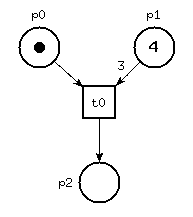
\includegraphics[height=40mm]{Red_Sensibilizada}}
    \subfigure[Disparo de $t_{0}$]{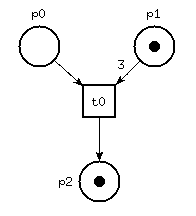
\includegraphics[height=40mm]{Red_Disparada}}
    \caption{Disparo de una transición}
    \label{fig:disparo_transicion}
  \end{figure}
  
  \item  [\underline{Definición 7}:] Matriz de Incidencia.\\
  La matriz de incidencia de una RdP se define como,
  $$ I = Post - Pre $$
  \textbf{Notas:}
  \begin{itemize}
    \item El disparo de una transición se reformula como, $$ m_{n+1}(p) =
    m_{n}(p) + I(p_{i}, t_{j}), \forall p_{i} \in P $$
    \item A partir de las matrices $Pre$ y $Post$ se puede reconstruir la
    estructura de la red, a partir de $I$ no es posible.
  \end{itemize}
\end{itemize}

\subsubsection{Sucesión de Disparos}

Si en lugar del disparo de una transición se requiere disparar múltiples
transiciones, se puede reescribir la ecuación de cambio de estado de la red de
la siguiente forma,
$$ m_{n+1} = m_{n} + I \times \sigma $$
En esta ecuación, $\sigma$ representa la sucesión de disparos a realizar. Se
cumple $\sigma \in \mathbb{N}^{t}$ y el elemento $\sigma_{i}$ contiene la
cantidad de disparos a realizar sobre $t_{i}$.\\
Si se comienza a realizar la sucesión de disparos $\sigma_{i}$ a partir del
marcado inicial $m_{0}$ y todos los disparos son exitosos, se llega a un marcado
$m_{i}$ y se dice que $m_{i}$ es \textit{alcanzable}.\\
De la misma forma, si existe un marcado $m_{j}$ alcanzable desde $m_{0}$, debe
exitir una sucesión de disparos $\sigma_{j}$ que permita alcanzarlo.

